% !TeX root = ./document.tex
\documentclass[document]{subfiles}
\begin{document}
\chapter{Теорема об открытом отображении}
\section{Обратные операторы}

$X,Y$ --- нормированные пространства, $A \in \Lin(X,Y)$. Уравнение $Ax = y$, где $y$ --- дано, $A$ --- дан, $x$ --- неизвестное.
Когда для $\forall y \in Y \: \exists! x \in X$ т.ч. $Ax = y \Rightarrow A$ --- биекция, то есть $\exists A^{-1}$. 

\[ \seq{y_n}^\infty_{n=1} \quad \liml_{n \to \infty} y_n = y \quad \exists! x_n : Ax_n = y_n \] 

Было бы хорошо, чтобы $x_n \underset{n \to \infty}{\longrightarrow} x, Ax = y$, то есть $A^{-1}$ --- непрерывен. Когда $\exists$ непрерывный $A^{-1}$?



Третий кит линейного функционального анализа будет как раз касаться обратных операторов. Понятно, что самый хороший оператор, который можно представить --- это тождественный, у него есть обратный, это он сам и есть.
 Вопрос такой: насколько можно отодвинуться от тождественного оператора, чтобы он остался обратимым?

\begin{theoremwobox}
    \begin{gather*}
        X \text{ --- банахово }, Ix = x, \: \forall x \in X \\
        \text{пусть } A \in \B(X), \norm{A} < 1 \Rightarrow \\
        \exists (I-A)^{-1} \in \B(X), \text{ при этом} \\
        (I-A)^{-1} = \sum^{+\infty}_{k=0} A^k (A^0 = i) \\
        \norm{(I-A)^{-1}} \leq \frac{1}{1 - \norm{A}}
    \end{gather*}
\end{theoremwobox}
% символическая картинка
\begin{proof}
    $X$ --- банахово $\Rightarrow \B(X)$ --- банахово. Был у нас критерий полноты, поэтому проверим, что ряд из норм сходится
    \begin{gather*}
        A, B \in \B(X) \Rightarrow \norm{AB} \leq \norm{A} \cdot \norm {B} \\
        \Rightarrow \norm{A^k} \leq \norm{A}^k \Rightarrow \sum^{+\infty}_{k=0} \norm{A^k} \leq \sum^{+\infty}_{k=0} \norm{A}^{k} = \frac{1}{1-\norm{A}}
        \Rightarrow \: \exists S = \sum^{+\infty}_{k=0} A^k, S \in \B(X) \\
        S_n = \sum^n_{k=0} A^k \Rightarrow \norm{S_n} \leq \frac{1}{1-\norm{A}} \Rightarrow \norm{S} \leq \frac{1}{1-\norm{A}}
     \end{gather*}
     проверим, что $S = (I-A)^{-1}$
     \begin{multline*}
        S_n(I-A) = (I + A + A^2 + \ldots + A^n)(I-A) = \\
        = (I-A) + (A-A^2) + \ldots + (A^n-A^{n+1}) = I - A^{n+1}
     \end{multline*}
     \begin{gather*}
        \norm{A^{n+1}} \leq \norm{A}^{n+1} \underset{n \to \infty}{\longrightarrow} 0 \Rightarrow \liml_{n \to \infty} (I-A^{n+1}) = I \\
        \Rightarrow \liml_{n \to \infty} S_n(I-A) = S(I-A) \Rightarrow S(I-A) = I \\
        (I-A)S_n = S_n(I-A) = I - A^{n+1} \Rightarrow \text{ при } n \to \infty \\
        (I-A)S = I \Rightarrow S (I-A)^{-1}
     \end{gather*}
\end{proof}

\begin{remark}
    $\dim X < +\infty, \: A,B \in \B(X), AB = I \Rightarrow B = A^{-1}$. Если $\dim X = +\infty$, то нет
\end{remark}

\begin{gather*}
    X = l^2, x = \seq{x_n}^\infty_{n=1}, x_n \in \bC, \norm{x}_2 = \left( \sum^\infty_{n=1} \abs{x_n}^2 \right)^{\frac{1}{2}} \\
    S(x) = (0, x_1, x_2, \ldots) \quad \norm{S} = 1, S \in \B(l^2) (S \text{ --- shift}) \\
    T(x) = (x_2, x_3, x_4, \ldots), \norm{T} = 1 \\
    (TS)(x) = x \Rightarrow TS = I \\
    \not \exists S^{-1} \text{ так как } S(l^2) \subsetneq l^2 \\
    \text{ то есть } \not \exists T^{-1}, T \text{ не инъективен}
\end{gather*}
Так что когда речь идёт о бесконечномерном пространстве, мы не зря проверили, что $AB = I, BA = I \Rightarrow B = A^{-1}$.


Применим эту теорему для общего случая, но сначала будет удобно ввести определение

\begin{definition}
    $X,Y$ --- нормированные 
    \[ \In(X,Y) = \seq{A \in \B(X,Y) : \: \exists A^{-1} \in \B(Y,X)} \]
\end{definition}

\begin{theorem}[множество обратных операторов открыто]
    $X$ --- банахово, $Y$ --- нормированное
    \begin{enumerate}
        \item \begin{gather*}
            A \in \In(X,Y) \\
            B \in \B(X,Y) \quad \norm{A-B} < \frac{1}{\norm{A^{-1}}} \Rightarrow B \in \In(X,Y) \text{ и при этом} \\
            \norm{B^{-1}} \leq \frac{\norm{A^{-1}}}{1 - \norm{AB} \cdot \norm{A^{-1}}} \tag{1} \\
            \norm{A^{-1} - \norm{B^{-1}}} \leq \frac{\norm{A-B} \cdot \norm{A^{-1}}^2}{1-\norm{AB}\cdot{A^{-1}}} \tag{2}
        \end{gather*}
        \item $\varphi: \In(X,Y) \rightarrow \In(Y,X) \quad \varphi(A) \coloneqq A^{-1} \Rightarrow \varphi \text{ непрерывное}$
    \end{enumerate}
\end{theorem}

\begin{proof}[1]
    \begin{gather*}
        \norm{A^{-1}(A-B)} \leq \norm {A^{-1}} \cdot \norm{A-B} < 1 \\
        \norm{W} < 1 \text{ по теореме об обратимости оператора, близкого к тождественному} \\
        \Rightarrow \: \exists (I-W)^{-1}, \norm{(I-W)^{-1}} \leq \frac{1}{1-\norm{W}} \leq \frac{1}{1-\norm{A^{-1}\cdot \norm{A-B}}} \\
        W = A^{-1}(A-B) = I - A^{-1}B \Rightarrow I - W = A^{-1} B \\
        B = A \cdot (A^{-1}B), \: \exists A^{-1}, \: \exists (A^{-1}B)^{-1} \Rightarrow \: \exists B^{-1} \\
        B^{-1} = (A^{-1}B)^{-1} \cdot A^{-1} \Rightarrow \\
        \norm{B^{-1}} \leq \norm{(A^{-1}B)^{-1}} \cdot \norm{A^{-1}} \leq \frac{\norm{A^{-1}}}{1-\norm{A^{-1}}\cdot \norm{A-B}} \tag{1}
    \end{gather*}
\end{proof}

Сейчас будет фантастический алгебраический трюк:
\begin{proof}[2]
    \begin{gather*}
        A^{-1} - B^{-1} = A^{-1}(B-A)B^{-1} \Rightarrow \\
        \norm{A^{-1} - B^{-1}} \leq \norm{A^{-1}} \cdot \norm{B-A} \cdot \norm{B^{-1}} \leq \frac{\norm{A-B} \cdot \norm{A^{-1}}^2}{1-\norm{A^{-1}} \cdot \norm{A-B}}
    \end{gather*}
\end{proof}

\begin{remark}
    Как мы можем истолковать первое утверждение?
    \[ B_{\frac{1}{\norm{A^{-1}}}}(A) \subset \In(X,Y) \]
    Как только есть обратимый, оператор, тогда шарик с центром в этом операторе и таким радиусом будет лежать в в множестве непрерывных операторов
\end{remark}

\begin{remark}
    \begin{gather*}
        \varphi(A) = A^{-1} \quad \varphi(B) = B^{-1} \\
        \norm{\varphi(A) - \varphi(B)} = \norm{A^{-1} - B^{-1}} \leq \frac{\norm{A-B} \cdot \norm{A^{-1}}^2}{1-\norm{A^{-1}} \cdot \norm{A-B}} \\
        \text{пусть } A \text{ фиксирован } \quad \liml_{B \to A} \norm{B-A} = 0 \Rightarrow \liml_{B \to A} \norm{\varphi(A) - \varphi(B)} = 0 \Rightarrow \\
        \Rightarrow \varphi \text{ непрерывное}
    \end{gather*}
\end{remark}


\section{Открытые отображения}

Определение касается только банаховых пространств, но дадим его в общем случае для произвольных топологических простанств

\begin{definition}[открытое отображение]
    $(X, \tau_1), (Y, \tau_2)$ --- топологические пространства. $U: X \rightarrow Y, U$ --- отображение.

    $U$ -- открытое, если $\forall G \subset X, G$ --- открытое $\Rightarrow U(G)$ --- открыто в $Y$
    
\end{definition}

\begin{remark}
    $U$ --- непрерывное, $G$ --- открытое $\Leftrightarrow (\forall G \subset Y \Rightarrow U^{-1}(G) \text{ открыт})$
\end{remark}

\begin{example}
    $f: \bR \rightarrow \bR, f(x) = \sin x \Rightarrow f(-\pi,\pi) = [-1,1]$, $f$ не лькоыьле
\end{example}

\begin{example}
    $f: [-\frac{\pi}{2}, \frac{\pi}{2}] \rightarrow \bR$, $f$ --- непрерывное, $f$ --- открытое, так как $\exists f^{-1}$ --- непрерывное
\end{example}


Открытость отображения, если есть обратное, означает непрерывность обратного отображения. Так и отметим в общем виде 

\begin{statement}
    $(X, \tau_1), (Y, \tau_2)$ --- топологические пространства, $U: X \rightarrow Y, U$ --- биекция 

    $U$ --- открытое $\Leftrightarrow U^{-1}$ --- непрерывно
\end{statement}
\begin{figure}
    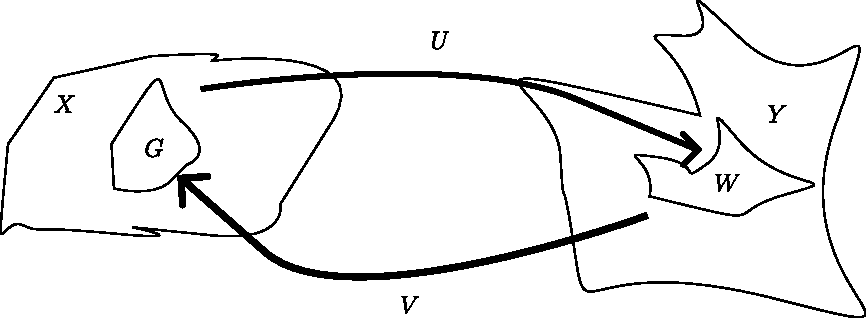
\includegraphics{chapter9/xygwuv.pdf}\caption{Утверждение 9.1}
\end{figure}
\begin{proof}
    \[V \coloneqq U^{-1} \quad X \stackrel{U}{\longrightarrow} Y \quad X \stackrel{V}{\longleftarrow} Y \]
    \[ W = U(G) \quad G = V(W) \quad W = V^{-1}(G) \] 
    $U$ --- открытое $\Leftrightarrow$ ($G$ --- открыто $\Rightarrow W = U(G)$ --- открыто).
    $V$ --- непрерывно $\Leftrightarrow (G$ --- открыто $\Rightarrow V^{-1}(G) = W$ --- открыт)
\end{proof}

\begin{statement}[критерий открытости линейного оператора]
    $(X, \norm{\cdot}, (Y, \norm{\cdot}))$ --- нормированные. $U \in \Lin(X,Y), U$ --- открытое
     $\Leftrightarrow \: \exists r > 0 B^Y_r(0) \subset U(B^X_1(0))$ (то есть $0 \in \Int(U(B_1(0))))$
\end{statement}

\begin{proof}
    $\Rightarrow$ \\
    $U$ --- открытое, $U(0) = 0, B^X_1(0)$ --- открытое $\Rightarrow U(B_1^X(0))$ --- открытое. 
    $0 \in U(B^X_1(0)) \Rightarrow \: \exists r > 0 B^Y_r(0) \subset U(B^X_1(0))$ \\
    $\Leftarrow$ \\
    Пусть $G \subset X, G$ --- открытое, $x_0 \in G \Rightarrow$ 
    \begin{gather*}
        \exists R > 0 \quad B^X_R(x_0) \subset G \\
        \Rightarrow B^Y_{rR}(0) \subset U(B^X_R(0))
        \intertext{Проверим, что $U(x_0)$ --- внутренняя точка $U(G)$}
        \underbrace{U(x_0) + B^Y_{rR}(0)}_{=B^Y_{rR}(U(x_0))} \subset U(x_0) + U(B^X_R(0)) = \\
        = U(B_R(x_0)) \subset U(G)
    \end{gather*}
\end{proof}

Перед тем, как доказывать главную теорему, ещё одно утверждение

\begin{statement}[необходимое условие открытости линейного оператора]
    $(X, \norm{\cdot}), (Y, \norm{\cdot})$ нормированные 
    \[ U \in \Lin(X,Y), U \text{ --- открытое } \Rightarrow U(X) = Y\]
\end{statement}


\begin{proof}
    \begin{gather*}
        \exists r > 0 \: B_r^Y(0) \subset U(B^X_1(0)) \Rightarrow B^Y_{rn}(0) \subset U(B^x_n(0)), n \in \bN \\
        \text{пусть } y \in Y \Rightarrow \: \exists n \in \bN : \norm{y} < nr \Rightarrow \\
        y \in B_{rn}(0) \subset U(B^X_n(0)) \subset U(X)
    \end{gather*}
\end{proof}


Вот и кит №3.

\begin{theorem*}[Банах, об открытом отображении]
    $(X, \norm{\cdot}), (Y, \norm{\cdot})$ --- банаховы, $U \in \B(X,Y)$. 
    Если $U(X) = Y$, то $U$ --- открытое
\end{theorem*}

Почему это кит? Потому что это очень полезный факт, на который постоянно хочется ссылаться.

Доказательсвто будет в 2 этапа. Сначала докажем лемму
\begin{lemma}[Редукция]
    $X$ --- банахово, $Y$ --- нормированное. Пусть $\exists r > 0, B_r^Y \subset \overline{U(B_1^X(0))}$ (замыкание) 
    \[ \Rightarrow B^Y_{\frac{r}{2}}(0) \subset U(B_1^X(0)) \]
\end{lemma}

\begin{proof}[Доказательство леммы]
    Поскольку $U$ --- линейное, то мы можем умножать на любую константу.
    \begin{gather*}
        \forall k \in \bN \quad B^Y_{\frac{r}{2^k}}(0) \subset \overline{U(B^X_{\frac{1}{2^k}}(0))} \\
        \text{пусть } y \in Y, \norm{y} < \frac{r}{2}
        \intertext{Построим $x, \norm{x} < 1$ т.ч. $Ux = y$. Будем его строить постепенно, сначала $x_1, x_2, \ldots$, и их сумма даст нам $x$}
        y \in B^Y_{\frac{r}{2}}(0) \subset \overline{U(B^x_{\frac{1}{2}}(0))} \Rightarrow \: \exists x_1, \norm{x_1} < \frac{1}{2} \\
        \norm{y-U(x_1)} \text{ может быть меньше, чем всё, что угодно, мы возьмум } \frac{r}{4} \\
        \norm{y-U(x_1)} < \frac{r}{4}, y - Ux_1 \in B^Y_{\frac{r}{4}}(0) \subset \overline{U(B^x_{\frac{1}{4}}(0))} \\
        \Rightarrow \: \exists x_2, \norm{x_2} < \frac{1}{4}, \norm{y-Ux_1-Ux_2} < 2 \frac{r}{2^3} \text{ и так далее} \\
        \seq{x_k}^\infty_{k=1}, \norm{x_k} < \frac{1}{2^k}, \norm{y-Ux_1- \ldots - Ux_k} < \frac{r}{2^{k+1}}\\
        \underbrace{\sum^\infty_{k=1} \norm{x_k}}_{\text{сходится}} < 1, [[\text{ банаховость X}]] \Rightarrow \\
        \exists x = \sum^\infty_{k=1} x_k, x \in X, \norm{x} < 1 \\
        S_n = \sum^n_{k=1} x_k \quad \liml_{n \to \infty} S_n = x \\
        \liml_{n \to \infty} \norm{y - US_n} = 0 \Rightarrow y = Ux, (U \text{ --- непрерывный})
    \end{gather*}
\end{proof}

\begin{proof}[Доказательство теоремы]
    \begin{gather*}
        B = B^X_1(0) \quad X = \bigcup^\infty_{n=1} nB, U(X) = Y \Rightarrow Y = \bigcup^\infty_{n=1} U(nB) \\
        Y \text{ --- банахово } [[\text{т. Бэра о категориях }]] \Rightarrow \: \exists n_0 : \Int(\overline{U(n_0B)}) \ne \varnothing \\
        U \text{ --- линейный } \Rightarrow \: \exists y_0 \in \Int(\overline{U(B)}) \Rightarrow \\
        \exists r > 0 \: B_r(y_0) \subset \overline{U(B)}
        \intertext{чтобы воспользоваться леммой, нам нужно заменить $y_0$ на $0$}
        \text{пусть } z \in Y, \norm{z} < r, y_0 + z \in \overline{U(B)} \\
        B \text{ --- симметричное множество, т.е. } x \in B \Rightarrow -x \in B \Rightarrow \\
        \overline{U(B)} \text{ --- симметричное, т.е. } y_0 \in \overline{U(B)} \Rightarrow -y_0 \in \overline{U(B)} \\
        z = (y_0 + z) + (-y_0) = \overline{U(B)} + \overline{U(B)} \subset \overline{U(2B)} \\
        \Rightarrow B_r^Y(0) \subset \overline{U(2B)} \Rightarrow B^Y_{\frac{r}{2}} \subset \overline{U(B)}  \\
        [[\text{ лемма о редукции }]] \Rightarrow B^Y_{\frac{r}{4}}(0) \subset U(B) [[\text{ критерий открытости }]] \Rightarrow \\
        U \text{ открыт}
    \end{gather*}
\end{proof}

Особенно часто применяется следствие, когда $U$ --- биекция
\begin{theorem*}[Банах, об обратном отображении]
    $X,Y$ --- банаховы, $U \in \B(X,Y), U \text{ --- биекция} \Rightarrow$
    \[ U^{-1} \in \B(Y,X) (\text{то есть } U^{-1} \text{ непрерывен}) \]
\end{theorem*}

Эта теорема нам пригодится, когда будем говорить о спектрах.

\section{Теорема об эквивалентных нормах и о замкнутом графике}

Когда мы говорили о нормах, нам обещалась некоторая сногсшибательная теорема, которую мы сейчас и докажем. 

\begin{theorem}
    $X$ --- линейное пространство, $\exists$ две нормы на $X$, т.ч. $(X, \norm{\cdot}_1), (Y, \norm{\cdot}_2)$ --- банаховы. 
    Пусть $\exists C > 0 : \norm{x}_2 \leq C \norm{X}_1 \forall x \in X$.
    Как бы это не могло показаться чудовищно странным, но существует и оценка в другую сторону
    \[ \Rightarrow \exists c_1 > 0 : \norm{x}_1 \leq c_1 \norm{x}_2 \: \forall x \in X \]
\end{theorem}

\begin{proof}
    Как мы уже делали, когда рассматривали 2 пространства с эквивалентными нормами, рассмотрим $X = (X, \norm{\cdot}_1), Y = (X, \norm{\cdot}_2)$
    \begin{gather*}
        Ix = x, I \in \Lin(X,Y), I \text{ --- биекция } \Rightarrow
        \norm{Ix}_2 \leq C \norm{x_1} \Rightarrow I \in \B(X,Y), \norm{I} \leq C \\
        [[\text{ т. Банаха об обратном отображении }]] \Rightarrow I^{-1} \in \B(Y,X) \Rightarrow \norm{x}_1 \leq c_1 \norm{x}_2 \: \forall x \in X
    \end{gather*}
\end{proof}

\begin{definition}[график]
    $X,Y$ --- нормированные,  над $\bC (\bR)$. $X \times Y $ --- линейное нормированное 
    \begin{gather*}
        (x,y) + (x_1,y_1) = (x+x_1,y+y_1), \lambda(x,y) = (\lambda x, \lambda y), \lambda \in \bC \\
        \norm{(x,y)}_{X \times Y} = \norm{x}_X + \norm{y}_Y \\
        U : X \rightarrow Y, U \text{ --- отображение } G_U = \seq{(x,Ux)}_{x \in X} \text{ --- график } U
    \end{gather*}
    $U$ --- замкнутое отображение, если $G_U$ --- замкнутое множество
\end{definition}

\begin{gather*}
    \Leftrightarrow (\liml_{n \to \infty} (x_n, Ux_n) = (x_0,y_0) \Rightarrow y_0 = Ux_0) \Leftrightarrow \\
    \left. \begin{matrix}
        \lim x_n = x_0 \\
        \lim Ux_n = y_0
    \end{matrix} \right\} \Rightarrow y_0 = Ux_0
\end{gather*}

Посмотрим, как связаны замкнутость и непрерывность. Мы убедимся, что замкнутость это более слабое утверждение (меньше), чем непрерывность.

\begin{remark}
    $U$ --- непрерывное $\Rightarrow U$ --- замкнутое
    \begin{enumerate}
        \item $\liml_{n \to \infty} x_n = x_0 $
        \item $\liml_{n \to \infty} Ux_n = y_0$
        \item $Ux_0 = y_0$
    \end{enumerate}
    $U \text{ непрерывен } \Leftrightarrow 1 \Rightarrow 2 + 3$; $U \text{ замкнутое } \Leftrightarrow 1 + 2 \Rightarrow 3$
\end{remark}

Есть множество примеров, где проверка замкнутости гораздо легче проверки непрерывности. И бывает иногда удобно, что эти условия равносильны.

\begin{theorem*}[о замкнутом графике]
    $X,Y$ --- банаховы, $U \in \Lin(X,Y), U$ --- замкнут $\Rightarrow U$ непрерывен
\end{theorem*}

\begin{proof}
    $(X, \norm{\cdot}_X), (Y, \norm{\cdot}_X)$. Новая  норма на $X$ : $\norm{x_1} = \norm{x}_X \norm{Ux}_Y$. Аксиомы нормы очевидны.

    Проверим, что $(X, \norm{\cdot}_1)$ --- банахово по определению
    \begin{gather*}
        \seq{x_n}^\infty_{n=1} \text{ фундаментальная в } (X_1, \norm{\cdot}_1), \text{ то есть } \\
        \underbrace{\norm{x_m-x_n}_1}_{\underset{m,n \to \infty}{\longrightarrow} 0} = \norm{x_m - x_n}_X + \norm{Ux_m - Ux_n}_{Y} \\
        \Rightarrow \liml_{m,n \to 0} X = 0 \Rightarrow 
        \intertext{Имеем дело с фундаментальными последовательностями в банаховом пространстве} 
        \left. \begin{matrix}
            \Rightarrow \: \exists x_0 \in X, \liml_{n \to \infty} x_n = x_0 \\ 
            \liml_{m,n\to 0} \norm{Ux_m - Ux_n}_Y = 0 \Rightarrow \: \exists y_0 \in Y \: \liml_{n \to \infty} Ux_n = y_0
        \end{matrix} \right\} \text{ замкнуто} \\
        \Rightarrow Ux_0 = y_0 \Rightarrow \\
        \liml_{n \to \infty} (\norm{x_n - x_0}_X + \norm{Ux_n - Ux_0}_Y) = 0 \\
        \Rightarrow (X, \norm{\cdot}_1) \text{ --- банахово} \\
        \Rightarrow \norm{x}_X \leq \norm{x}_X + \norm{Ux}_Y = \norm{x}_1 \\
        [[\text{ теорема об эквивалентных нормах}]] \Rightarrow \\
        \exists c_0 \quad \norm{x}_X + \norm{Ux}_Y \leq C \norm{x}_X \Rightarrow \norm{Ux}_Y \leq C \norm{x}_X \Rightarrow U \in \B(X,Y)
    \end{gather*}
\end{proof}

Естественно, требются примеры, когда есть замкнутость, но нет непрерывности.
\begin{remark}
    $X,Y$ --- нормированные, $U \in \Lin(X,Y)$, $U \not \Rightarrow U$ --- непрерывный. 
\end{remark}

У нас было не так много не непрерывных операторов: например, оператор дифференцирования, им и воспользуемся.
\begin{example}
    \begin{gather*}
        D(f) = f^\prime, Y = C[-1,1], X \subset Y, X = \seq{f: f\prime \in C[-1,1]} \\
        \norm{f}_X = \norm{f}_Y = \max_{x \in [-1,1]} \abs{f(x)} \\
        D(x^n) = nx^{n-1}, \norm{D(x^n)} = n, \norm{x^n} = 1 \Rightarrow \sup_{\norm{f} = 1} \norm{D(f)} = +\infty \\
        \Rightarrow D \text{ не непрерывен}
        \intertext{это воспоминание о не непреывности. Почему же он замкнут?}
        \seq{f_n}^\infty_{n=1}, f_n \in X, f_n \stackrel{X}{\longrightarrow} f, D(f_n) \stackrel{Y}{\longrightarrow} g \stackrel{?}{\Rightarrow} [[\text{ замкнутость }]] D(f) = g \\
        \intertext{когда-то в анализе доказали}
        \left. \begin{matrix}
            f_n \darrow{[-1,1]} f \\
            f^\prime_n \darrow{[-1,1]} g
        \end{matrix} \right\} \Rightarrow g = f^\prime, \text{то есть } D(f) = g \Rightarrow D \text{ замкнут}
    \end{gather*}
\end{example}

Теорему о замкнутости графика нельзя применять, потому что $X$ --- не полное. Более того, $\overline{X} = Y$

\section{Примеры неограниченных операторов в банаховом пространстве}

Заодно ещё раз вспомним лемму Цорна, чтобы мы не думали, что это была экзотика для доказательства теоремы Хана-Банаха, а вполне рабочий инструмент, когда мы хотим постриоть максимальный элемент
в бесконечных множествах, где обычная индукция не помогает.
\begin{definition}[алгебраический базис]
    $X$ --- линейное пространств над $\bC$ (или $\bR$). $\seq{x_\alpha}_{\alpha \in A}$ --- \textbf{алгебраический базис} (базис Гамеля), если 
    $\forall x, x = \sum^n_{j=1} c_j x_{\alpha_j}$ такое представление единственно.
\end{definition}
В конечномерном пространстве разницы с предыдущим определением базиса нет. Но в бесконечномерных пространствах на конечное представление надежды нет.

\begin{theorem}
    $X$ --- линейное пространство $\Rightarrow$ в $X \: \exists$ базис Гамеля.
\end{theorem}

\begin{proof}
    План такой: мы возьмём максимальное линейно-независимое множество и назовём его максимальным элементом, потом применим лемму Цорна. 
    Когда мы говорим о линейной независимости, речь идёт только о конечных комбинациях
    \begin{gather*}
        \Rho = \seq{Y: Y \subset x, Y \text{ --- линейно независимое }} \\
        \text{порядок } Y \leq Z, \text{ если } Y \subset Z, \: Y,Z \in \Rho
        \intertext{для того, чтобы применить лемму Цорна, нужно установить, что в любом линейно упорядоченном множестве есть верхняя грань}
        \seq{Y_\alpha}_{\alpha \in A} \text{ --- линейно упорядоченное множество, то есть} \\
        \forall \alpha, \beta \text{ либо } Y_{\alpha} \subset Y_{\beta} \text{ или } Y_\beta \subset Y_\alpha \\
        Y_0 = \bigcup_{\alpha \in A} Y_\alpha \Rightarrow Y_0 \text{ --- верхняя грань для } \seq{Y_\alpha}_{\alpha \in A} \\
        [[\text{ лемма Цорна }]] \Rightarrow \text{ в } \Rho \: \exists \text{ максимальный элемент } Z
        \intertext{проверим, что $\calL(Z) = X$. Допустим $\exists x_0 \in X \setminus \calL(Z)$} 
        Y = x_0 \cup Z \Rightarrow Y \subset \Rho, Z \leq Y, Z \ne Y \\
        \text{противоречие } \Rightarrow Z \text{ --- базис Гамеля}
    \end{gather*}
    
\end{proof}

С помощью этого базиса построим примеры, если их вообще можно назвать примерами, ведь они будут совсем-совсем неявными.
\begin{example}
    $X$ --- банахово, $\dim X = \infty$, пусть $\seq{x_\alpha}_{\alpha \in A}$ --- базис Гамеля
    \begin{gather*}
        \seq{\lambda_\alpha}_{\alpha \in A}, \lambda_{\alpha} \in \bC \quad \sup_{\alpha \in A} \abs{\lambda_\alpha} = +\infty \\
        U: X \rightarrow X, U(x_\alpha) = \lambda_\alpha \cdot x_\alpha
        \intertext{по линейности продолжим}
        x \in X \Rightarrow x = \sum^n_{j=1} c_j x_{\alpha_j} \quad U(x) = \sum^n_{j=1} c_j \lambda_{\alpha_j} x_{\alpha_j} \\
        U \in \Lin(X), \sup_{\alpha \in A} \frac{\norm{U(x_\alpha)}}{\norm{x_\alpha}} = \sup_{\alpha \in A} \abs{\lambda_\alpha} = +\infty \Rightarrow U \notin \B(x)
    \end{gather*}
\end{example}

Пример не очень явный, но, тем не менее, вот такие ужасы. Теперь пусть будет не непрерывный линейный функционал.

\begin{example}
    $X$ --- банахово, $\seq{x_\alpha}_{\alpha \in A}$ --- базис Гамеля, $\seq{\lambda_\alpha}_{\alpha \in A}, \sup_{\alpha \in A} \abs{\lambda_\alpha} = +\infty$
    \begin{gather*}
        f: X \rightarrow \bC \quad f(x_\alpha) = \lambda_\alpha \cdot \norm{x_\alpha}
        \intertext{продолжим по линейности}
        \Rightarrow f \in \Lin(X, \bC), \sup_{\alpha} \frac{\abs{f(x_\alpha)}}{\norm{x_\alpha}} = +\infty \Rightarrow f \notin X^*
    \end{gather*}
\end{example}

\begin{example}
    \begin{gather*}
        l^2, \seq{e_n}^\infty_{n=1}, e_n = (0, \ldots, 0, \underbrace{1}_n, 0, \ldots) \\
        \Rho 9 \seq{Y \subset l^2, E = \seq{e_n}^\infty_{n=1}}, E \subset Y, Y \text{ --- линейно независимое} \\
        \exists \text{ максимальный элемент} \\
        \seq{e_\alpha}_{\alpha \in A} \text{ --- базис Гамеля} \\
        \bN \subset A, \lambda_n = n, \text{ то есть } \\
        f(e_n) = n, f(e_\alpha) = \lambda_\alpha, \lambda_\alpha \in \bC, \lambda_{\alpha} \text{ --- любое} \\
        \sup_n \abs{f(e_n)} = +\infty \Rightarrow f \notin (l^2)^\infty \text{ при } \alpha \ne n
    \end{gather*}
\end{example}

\end{document}
